% Chapter X

\chapter{Results} % Chapter title
\label{ch:results} % For referencing the chapter elsewhere, use \autoref{ch:name} 

This chapter is dedicated to the description of the OCT software that was developed for this thesis. This application handles the data acquisition task, controls the galvanometric system and performs real-time processing and visualization of the acquired OCT data. \\

\noindent The transversal resolution of the system described in \autoref{ch:setup} is also evaluated using the test resolution target introduced in the same chapter. \\

\noindent Finally, a series of B-scans, C-scans and \emph{en-face} images of a variety of different samples is presented. A part of these were acquired using a second SS-OCT system designed to work in the 1060 nm range. 


%----------------------------------------------------------------------------------------

\section{Data Acquisition Software}

The final component that is needed to obtain a working SS-OCT system is a computer application that handles data acquisition and image visualization. This program should be able to achieve real-time performances, enabling a low-delay video stream of cross-sectional OCT data. Ideally, the total acquisition rate of the system in terms of B-scan/s should be limited by the scanning speed of the galvanometric mirrors and not by the OCT software. In fact, given the transversal resolution of the system, the FOV of the scanning lens and the spot size on the focal plane, there exists a maximum frequency at which the mirrors can be driven in order to obtain distortion-free images. An extensive analysis on this matter is carried out in \cite{Calabrese2017}. \\


%Leave this chapter for the explanation of the software, technologies used, performance achieved and showcase of the measurements. B-scans, volumes and enface. Also include control of the galvo mirrors in here since it's about C++ programming. 

%Explain in detail the fact that for real time the average time to process has to be < frame time and explain buffer ring to get buffer from board using DMA. Check datasheet in the pdfviwer since there is a nice explanation of async drivers. 

\noindent The application is developed for the Windows 10 Operating System using the Object-Oriented C++ programming language, which is the only one that allows low-level memory management among those supported by the ATS9350 acquisition board. Additionally, it permits the native integration of the high performance graphics library called OpenGL\footnote{\url{https://www.opengl.org/}}. \\


The code is built using the Qt application framework\footnote{\url{https://www.qt.io/}}, which consists in a set of tools for event handling and the design of \acp{GUI}. In Qt, asynchronous code can be easily written using the Signals and Slots paradigm: when a particular event occurs, an object \emph{emits} a signal; objects that are connected to this signal will execute the appropriate slot, which is a function that takes the parameters passed by the emitted signals and perform some actions. For example, the object dealing with OCT data acquisition can emit a signal with a newly acquire B-scan, while a data visualization object connected to this signal can retrieve this data and display it without blocking the acquisition task. 


\subsection{Controlling the galvanometric mirrors}

\subsection{Programming the ATS9350 board}


\subsection{Performance results}


\subsection{Displaying graphics with OpenGL}

\subsection{Parallel Computing with OpenMP}
OpenMP\footnote{\url{http://www.openmp.org/}} \graffito{OpenMP stands for Open \textbf{M}ulti-\textbf{P}rocessing} is a multi-platform \emph{Application Programming Interface} (API) for shared-memory parallel processing programming available for various programming languages, such as C, C++ and Fortran. 


\subsection{Amplified Photodiode}



\begin{figure}[hbt]
	\centering
	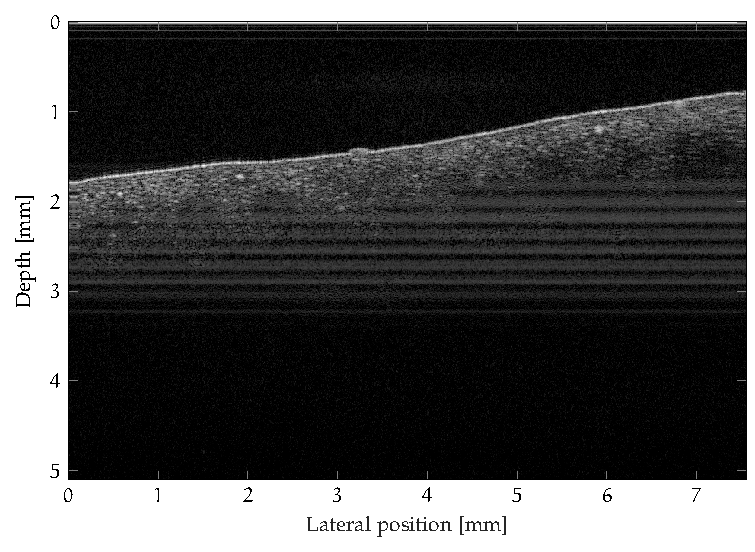
\includegraphics[width=\linewidth]{gfx/tikz/axsun/banana-peel}
	\caption{B-scan of banana peel.}\label{fig:banana-peel}
\end{figure}%----------------------------------------------------------------------------------------
\begin{figure}[hbt]
	\myfloatalign
	{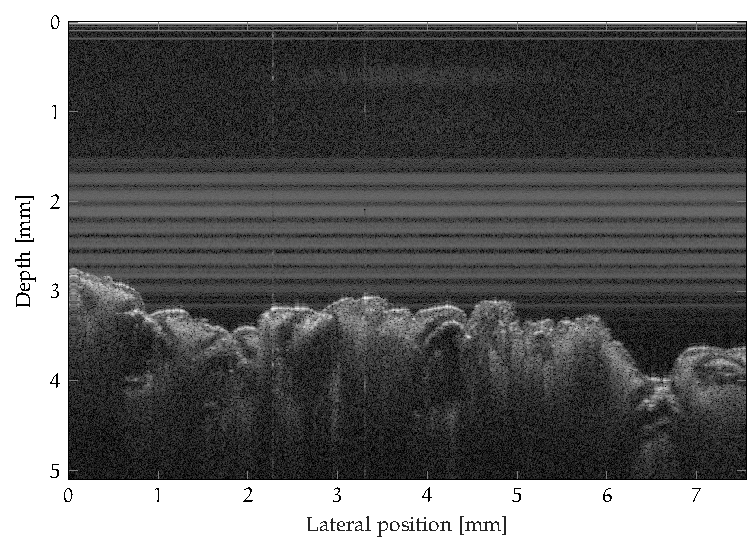
\includegraphics[width=\linewidth]{gfx/tikz/axsun/dry-orange-peel}}
	\caption{B-scan of dry orange peel.}\label{fig:dry-orange-peel}
\end{figure}%----------------------------------------------------------------------------------------

\begin{figure}[hbt]
	\myfloatalign
	{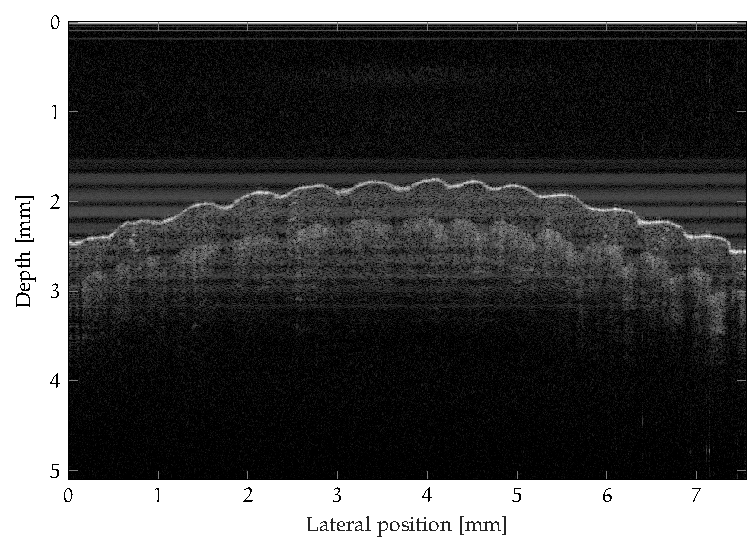
\includegraphics[width=\linewidth]{gfx/tikz/axsun/finger}}
	\caption{B-scan of a human finger.}\label{fig:finger}
\end{figure}%----------------------------------------------------------------------------------------
%----------------------------------------------------------------------------------------


\begin{figure}[hbt]
\myfloatalign
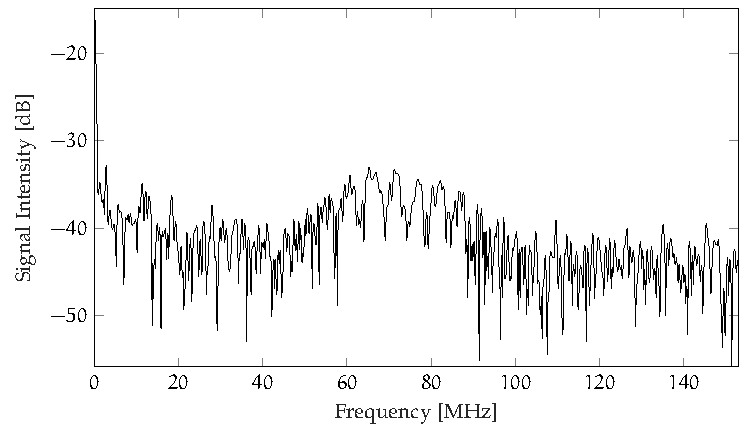
\includegraphics[width=\linewidth]{gfx/tikz/axsun/spurious-frequencies}
\caption{Spurious beat frequencies detected by the Exalos \ac{BPD}.}\label{fig:spurious-frequencies}
\end{figure}%----------------------------------------------------------------------------------------


Content

%----------------------------------------------------------------------------------------

\section{Galvanometric System Control}
	\begin{enumerate}
		\item NI-DAQmx framework
		\item C programming
		\item Triggering and Clocking
		\item Splitting Positive and Negative voltages
		\item Conversion from volts to angles to surface area
		\item Trigger enable
		\item X-Motor -> Triangle Wave
		\item Y-Motor -> Staircase for C-scans		
	\end{enumerate}





\begin{figure}[bth]
	\myfloatalign
	\subfloat[Asia personas duo.]
	{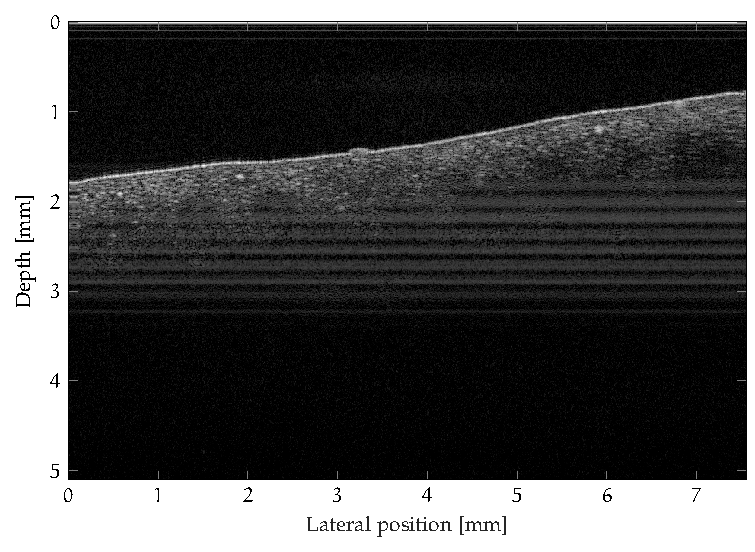
\includegraphics[width=.45\linewidth]{gfx/tikz/axsun/banana-peel}} \quad
	\subfloat[Pan ma signo.]
	{\label{fig:banan-peel}
		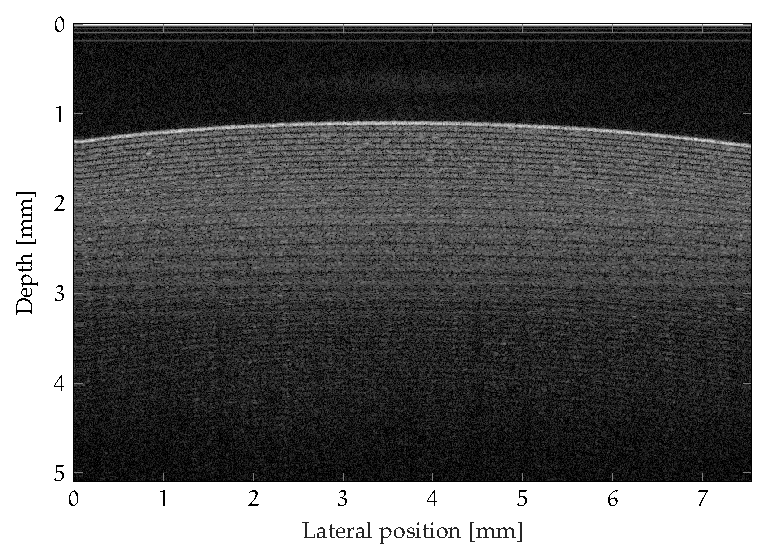
\includegraphics[width=.45\linewidth]{gfx/tikz/axsun/tape}} \\
	\subfloat[Methodicamente o uno.]
	{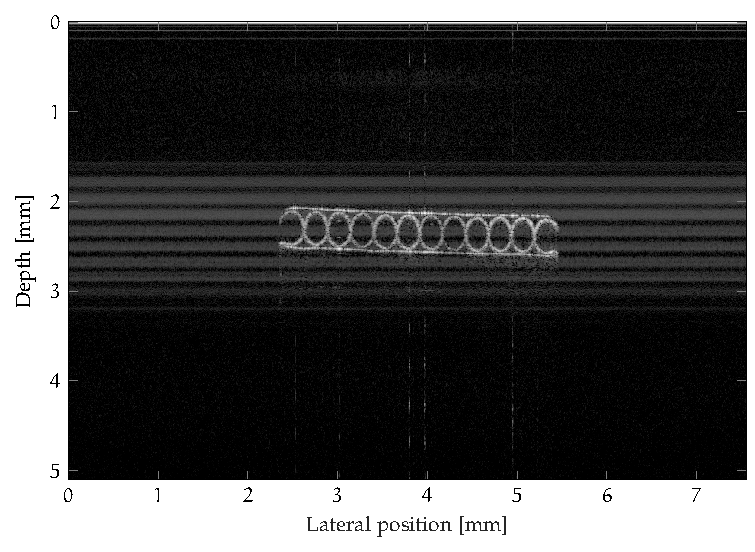
\includegraphics[width=.45\linewidth]{gfx/tikz/axsun/nastro}} \quad
	\subfloat[Titulo debitas.]
	{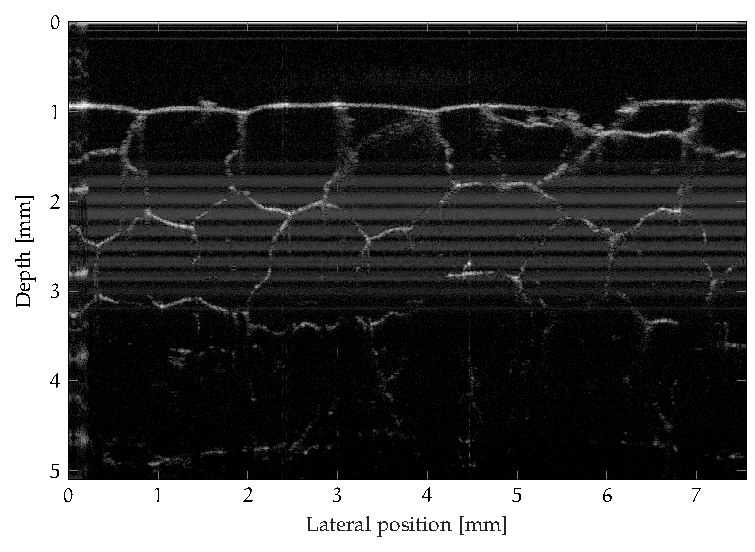
\includegraphics[width=.45\linewidth]{gfx/tikz/axsun/spugna-1}}
	\caption{Tu duo titulo debitas latente.}\label{fig:example}
\end{figure}


\section{USAF Target}
    \begin{figure}[hbt]
        \centering
        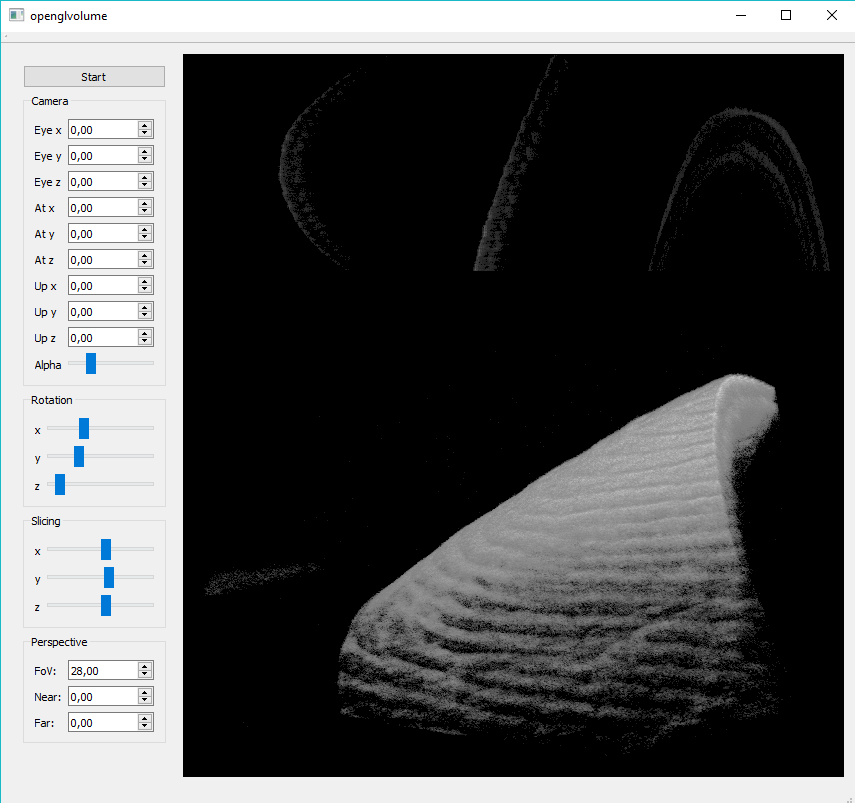
\includegraphics[width=0.8\linewidth]{gfx/3d/finger}
        \caption[]{3D rendering of a human finger.}\label{fig:finger-3d}
    \end{figure}

	\begin{figure}[hbt]
		\centering
		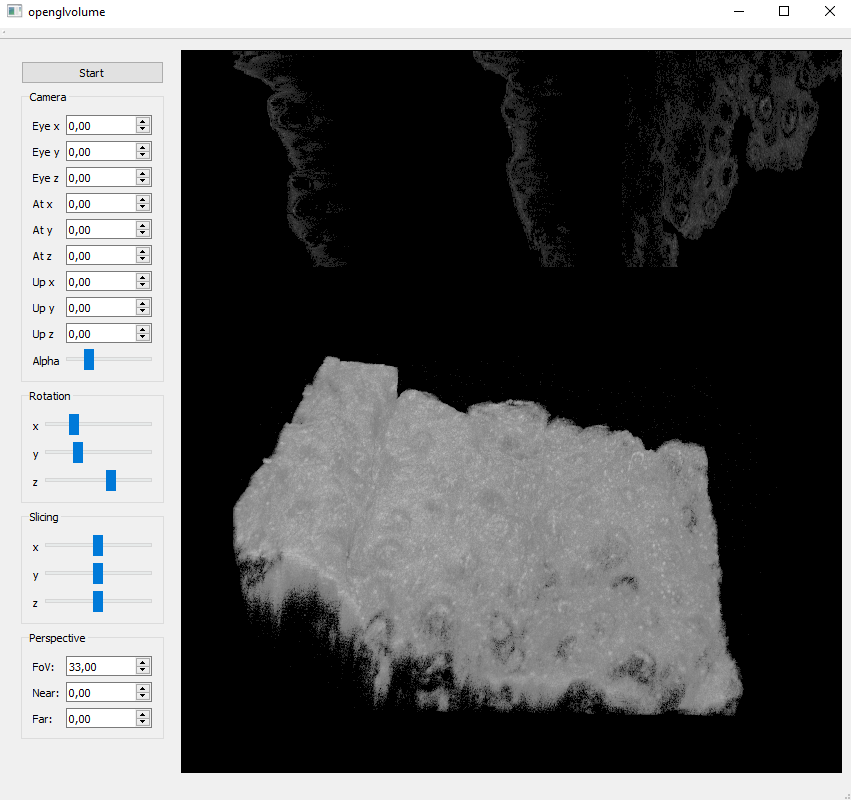
\includegraphics[width=0.8\linewidth]{gfx/3d/dry-orange}
		\caption[]{3D rendering of a human finger.}\label{fig:orange-3d}
	\end{figure}

    \begin{figure}[hbt]
        \centering
        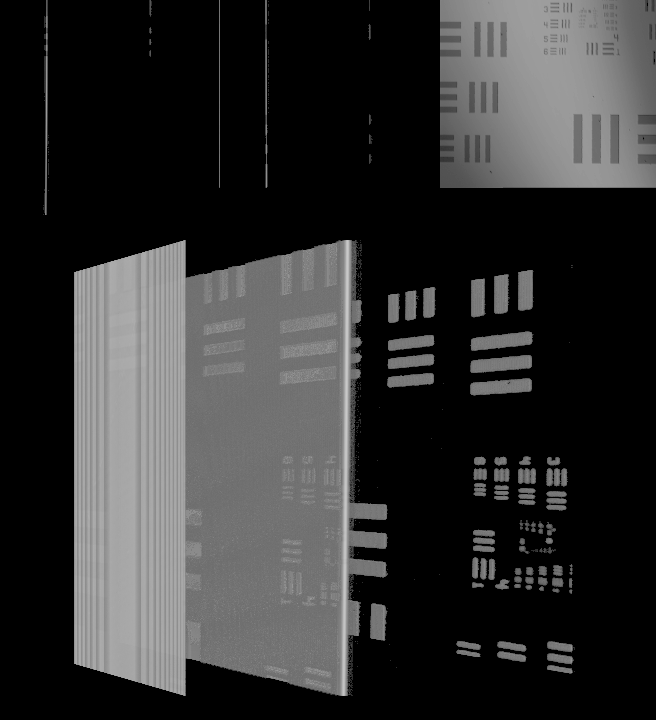
\includegraphics[width=1\linewidth]{gfx/3d/target}
        \caption[]{3D rendering of the USAF target}\label{fig:targer-3d}
    \end{figure}

	\begin{enumerate}
		\item What it is
		\item How it works
		\item Acquisitions in different conditions
		\item B-scans
		\item Surface images -> verifying transverse resolution
	\end{enumerate}

Content
